%[a4paper]


\documentclass{article}
%%%%%%%%%%%%%%%%%%%%%%%%%%%%%%%%%%%%%%%%%%%%%%%%%%%%%%%%%%%%%%%%%%%%%%%%%%%%%%%%%%%%%%%%%%%%%%%%%%%%%%%%%%%%%%%%%%%%%%%%%%%%%%%%%%%%%%%%%%%%%%%%%%%%%%%%%%%%%%%%%%%%%%%%%%%%%%%%%%%%%%%%%%%%%%%%%%%%%%%%%%%%%%%%%%%%%%%%%%%%%%%%%%%%%%%%%%%%%%%%%%%%%%%%%%%%
\usepackage{amsfonts}
\usepackage{amsmath}
\usepackage{fullpage}
\usepackage{graphicx}
\usepackage{subfigure}
\usepackage{color,hyperref,cite}

\setcounter{MaxMatrixCols}{10}
%TCIDATA{OutputFilter=LATEX.DLL}
%TCIDATA{Version=5.50.0.2890}
%TCIDATA{<META NAME="SaveForMode" CONTENT="1">}
%TCIDATA{BibliographyScheme=BibTeX}
%TCIDATA{Created=Monday, September 27, 2010 21:32:20}
%TCIDATA{LastRevised=Monday, January 09, 2023 13:19:17}
%TCIDATA{<META NAME="GraphicsSave" CONTENT="32">}
%TCIDATA{<META NAME="DocumentShell" CONTENT="Standard LaTeX\Blank - Standard LaTeX Article">}
%TCIDATA{Language=American English}
%TCIDATA{CSTFile=40 LaTeX article.cst}

\sloppy
\newtheorem{theorem}{Theorem}
\newtheorem{acknowledgement}{Acknowledgement}
\newtheorem{algorithm}{Algorithm}
\newtheorem{axiom}{Axiom}
\newtheorem{case}{Case}
\newtheorem{claim}{Claim}
\newtheorem{conclusion}{Conclusion}
\newtheorem{condition}{Condition}
\newtheorem{conjecture}{Conjecture}
\newtheorem{corollary}{Corollary}
\newtheorem{criterion}{Criterion}
\newtheorem{definition}{Definition}
\newtheorem{observation}{Observation}
\newtheorem{example}{Example}
\newtheorem{exercise}{Exercise}
\newtheorem{lemma}{Lemma}
\newtheorem{notation}{Notation}
\newtheorem{researchproblem}{Research Problem}
\newtheorem{proposition}{Proposition}
\newtheorem{remark}{Remark}
\newtheorem{solution}{Solution}
\newtheorem{summary}{Summary}
\newtheorem{assumption}{Assumption}
\newenvironment{proof}[1][Proof]{\noindent\textbf{#1.} }{\ \rule{0.5em}{0.5em}}
\newenvironment{proofofclaim}[1][Proof]{\noindent\textbf{#1.} }{\ensuremath{\square}}


\begin{document}
	
	
	\begin{remark}
		In the following, we only consider \emph{wasteless} temporal paths. A
		temporal path $P=((e_{1},t_{1}),\ldots ,(e_{k},t_{k}))$ is \emph{wasteless}
		if, for every $i=1,2,\ldots ,k-1$, we have that $t_{i+1}$ is the first time
		after $t_{i}$ that the edge $e_{i+1}$ appears.
	\end{remark}
	
	\begin{definition}
		\label{arrival-duration-def}Let $u,v\in V$, and let $t\in 
		%TCIMACRO{\U{2115} }%
		%BeginExpansion
		\mathbb{N}
		%EndExpansion
		$. Given that a temporal path starts within the period $[t,t+\Delta -1]$,
		the \emph{arrival} of the fastest path in $(G,\lambda )$ from $u$ to $v$ is $%
		A_{t}(u,v)$, and the \emph{arrival} along path $P$ in $(G,\lambda )$ from $u$
		to $v$ is $A_{t}(u,v,P)$.
	\end{definition}
	
	Whenever $t=1$, we may omit the index $t$, i.e. we may write $%
	A(u,v,P)=A_{1}(u,v,P)$ and $A(u,v)=A_{1}(u,v)$. The following refers to
	Figure~\ref{conj-fig}.
	
	Initial assumptions:
	
	\begin{enumerate}
		\item $d(u_{0},u_{i})=d(u_{0},u_{i},P)\leq d(u_{0},u_{i},Q)$; denote $\delta
		_{0}=d(u_{0},u_{i},Q)-d(u_{0},u_{i})\geq 0$.
		
		\item $d(u_{0},u_{k})=d(u_{0},u_{k},Q\cup R)\leq d(u_{0},u_{k},P\cup R)$.
	\end{enumerate}
	
	General properties:
	
	\begin{itemize}
		\item $A_{t}(u,v,P)=t_{0}+d(u,v,P)-1$, for every $u,v$, where $t_{0}\in
		\lbrack t,t+\Delta -1]$ is the label of the first edge of the path $P$ from $%
		u$ to $v$.
	\end{itemize}
	
	\bigskip
	
	Let $t_{u_{1}}\in \lbrack 1,\Delta ]$ be the label of the edge $u_{0}u_{1}$,
	and denote by $t_{v_{1}}$ the appearance of the edge $u_{0}v_{1}$ within the
	period $[t_{u_{1}},t_{u_{1}}+\Delta -1]$. Note that $1\leq t_{u_{1}}\leq
	\Delta $ and that $t_{u_{1}}\leq t_{v_{1}}\leq 2\Delta $. By the first
	initial assumption, we have:
	
	\begin{equation*}
		\delta
		_{0}=d(u_{0},u_{i},Q)-d(u_{0},u_{i})=A_{t_{u_{1}}}(u_{0},u_{i},Q)-A_{t_{u_{1}}}(u_{0},u_{i},P)+\left( t_{v_{1}}-t_{u_{1}}\right)
	\end{equation*}%
	and thus%
	\begin{equation}
		A_{t_{u_{1}}}(u_{0},u_{i},P)-A_{t_{u_{1}}}(u_{0},u_{i},Q)=t_{v_{1}}-(t_{u_{1}}+\delta _{0})
		\label{basic-eq-1}
	\end{equation}
	
	\begin{lemma}
		\label{lem-1}If $t_{v_{1}}\neq t_{u_{1}}$ then $\delta _{0}\leq \Delta -2$
		and $t_{v_{1}}\geq t_{u_{1}}+\delta _{0}+1$.
	\end{lemma}
	
	\begin{proof}
		First assume that $\delta _{0}\geq \Delta -1$. Then, it follows by (\ref%
		{basic-eq-1}) that $%
		A_{t_{u_{1}}}(u_{0},u_{i},P)-A_{t_{u_{1}}}(u_{0},u_{i},Q)\leq
		t_{v_{1}}-t_{u_{1}}-\Delta +1\leq 0$, and thus $A_{t_{u_{1}}}(u_{0},u_{i},P)%
		\leq A_{t_{u_{1}}}(u_{0},u_{i},Q)$. Therefore, since we can traverse path $P$
		from $u_{0}$ to $u_{i}$ by departing at time $t_{v_{1}}\geq t_{u_{1}}+1$ and
		by arriving no later than traversing path $Q$, we have that $d(u_{0},u_{k},P\cup Q)<d(u_{0},u_{k},Q\cup R)$, which is a contradiction to the
		second initial assumption. Therefore $\delta _{0}\leq \Delta -2$.
		
		Now assume that $t_{u_{1}}+1\leq t_{v_{1}}\leq t_{u_{1}}+\delta _{0}$. Then,
		it follows by (\ref{basic-eq-1}) that $A_{t_{u_{1}}}(u_{0},u_{i},P)\leq
		A_{t_{u_{1}}}(u_{0},u_{i},Q)$ which is, similarly to the previous case, a
		contradiction. Therefore $t_{v_{1}}\geq t_{u_{1}}+\delta _{0}+1$.
	\end{proof}
	
	\medskip
	
	The next corollary follows immediately from Lemma \ref{lem-1}.
	
	
	\begin{corollary}
		\label{cor-1}If $t_{v_{1}}\neq t_{u_{1}}$ then $1\leq
		A_{t_{u_{1}}}(u_{0},u_{i},P)-A_{t_{u_{1}}}(u_{0},u_{i},Q)\leq \Delta
		-1-\delta _{0}$.
	\end{corollary}
	
	\begin{lemma}
		\label{lem-2}$d(u_{0},u_{i-1},P\cup \{u_{i}u_{i-1}\})>d(u_{0},u_{i-1},Q\setminus
		\{u_{i}u_{i-1}\})$.
	\end{lemma}
	
	\begin{proof}
		Let $e\in \lbrack 1,\Delta ]$ be the label of the edge $u_{i-1}u_{i}$, and
		let $f\in \lbrack e+1,e+\Delta ]$ be the time of the first appearance of the
		edge $u_{i}u_{i+1}$ after time $e$. Let $A_{t_{u_{i}}}(u_{0},u_{i},Q)=x%
		\Delta +e$. Then $A_{t_{u_{i}}}(u_{0},u_{i+1},Q\cup\{u_{i}u_{i+1}\})=x\Delta +f$. Furthermore let $g$ be such
		that $A_{t_{u_{i}}}(u_{0},u_{i},P)=x\Delta +g$. 
		
		\emph{Case 1: }$t_{v_{1}}\neq t_{u_{1}}$\emph{.} Then Corollary \ref{cor-1}
		implies that $e+1\leq g\leq e+(\Delta -1-\delta _{0})$. Assume that $g<f$.
		Then, we can traverse path $P$ from $u_{0}$ to $u_{i}$ by departing at time $%
		t_{v_{1}}\geq t_{u_{1}}+1$ and by arriving at most at time $x\Delta +f-1$,
		and thus $d(u_{0},u_{k},P\cup R)<d(u_{0},u_{k},Q\cup R)$, which is a
		contradiction to the second initial assumption. Therefore $g\geq f$. That is,%
		\begin{equation}
			e+1\leq f\leq g\leq e+(\Delta -1-\delta _{0}).  \label{basic-eq-2}
		\end{equation}
		
		Consider the path $P^{\ast }=P\cup \{u_{i}u_{i-1}\}$. Assume that we start
		traversing $P^{\ast }$ at time $t_{v_{1}}$. Then we arrive at $u_{i}$ at
		time $x\Delta +g$, and we continue by traversing edge $u_{i}u_{i-1}$ at time 
		$(x+1)\Delta +e$. That is, $d(u_{0},u_{i-1},P^{\ast })=(x+1)\Delta
		+e-t_{v_{1}}+1$. 
		
		Now consider the path $Q^{\ast }=Q\setminus \{u_{i}u_{i-1}\}$. Let $h\in
		\lbrack 1,\Delta ]$ be such that $A_{t_{u_{i}}}(u_{0},u_{i-1},Q^{\ast
		})=x\Delta +e-h$. That is, if we start traversing $Q^{\ast }$
		at time $t_{u_{1}}$, we arrive at $u_{i-1}$ at time $x\Delta +e-h$, i.e. $%
		d(u_{0},u_{i-1},Q^{\ast })=x\Delta +e-h-t_{u_{1}}+1$. Summarizing, we have:%
		\begin{eqnarray*}
			d(u_{0},u_{i-1},P^{\ast })-d(u_{0},u_{i-1},Q^{\ast }) &=&\Delta
			+h-(t_{v_{1}}-t_{u_{1}}) \\
			&\geq &(\Delta -\delta _{0})+h>0,
		\end{eqnarray*}%
		which proves the statement of the lemma.
		
		\emph{Case 2: }$t_{v_{1}}=t_{u_{1}}$\emph{.} Then, it follows by (\ref%
		{basic-eq-1}) that $%
		A_{t_{u_{1}}}(u_{0},u_{i},P)=A_{t_{u_{1}}}(u_{0},u_{i},Q)-\delta _{0}\leq
		A_{t_{u_{1}}}(u_{0},u_{i},Q)$. Therefore $g\leq e$. Similarly to Case 1
		above, consider the paths $P^{\ast }=P\cup \{u_{i}u_{i-1}\}$ and $Q^{\ast
		}=Q\setminus \{u_{i}u_{i-1}\}$. Assume that we start traversing $P^{\ast }$
		at time $t_{v_{1}}=t_{u_{1}}$. Then we arrive at $u_{i}$ at time $x\Delta +g$%
		, and we continue by traversing edge $u_{i}u_{i-1}$, either at time $%
		(x+1)\Delta +e$ (in the case where $g=e$) or at time $x\Delta +e$ (in the
		case where $g\neq e$). That is, $d(u_{0},u_{i-1},P^{\ast })\geq x\Delta
		+e-t_{u_{1}}+1$.
		
		Similarly to Case 1, let $h\in \lbrack 1,\Delta ]$ be such that $%
		A_{t_{u_{i}}}(u_{0},u_{i-1},Q^{\ast })=x\Delta +e-h$. That is, if we start
		traversing $Q^{\ast }$ at time $t_{u_{1}}$, we arrive at $u_{i-1}$ at time $%
		x\Delta +e-h$, i.e. $d(u_{0},u_{i-1},Q^{\ast })=x\Delta +e-h-t_{u_{1}}+1$.
		Summarizing, we have:%
		\begin{equation*}
			d(u_{0},u_{i-1},P^{\ast })-d(u_{0},u_{i-1},Q^{\ast })\geq h\geq 1,
		\end{equation*}%
		which proves the statement of the lemma.
	\end{proof}
	
	\medskip
	
	\begin{figure}[htbp]
		\centering
		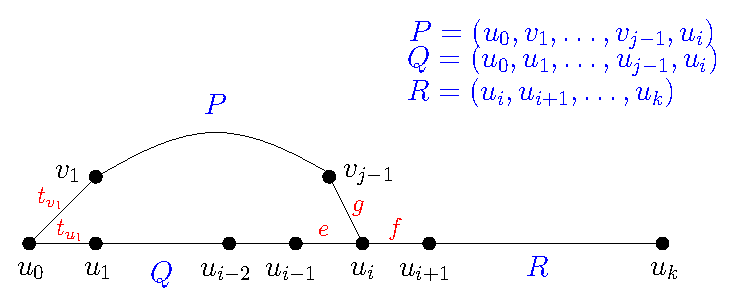
\includegraphics[width=0.6\linewidth]{conj-fig}
		\caption{Figure of the conjecture.}
		\label{conj-fig}
	\end{figure}
	
	%
	%
	%{\small 
		%\bibliographystyle{abbrv}
		%\bibliography{ref-evolution}
		%}
	
\end{document}
